% !TeX root = ../../Book1.tex
% 纲要标题：### 3.3 多面体的两种表示与对偶
% 纲要位置：几何学计划纲要.md，第 218 行。
% 正文状态：初稿；尚未正式审核。

% 纲要内容开始
% 
% * 半空间表示与顶点表示
% * 有界多面体的等价描述
% * 面、法锥与面格
% * 极体及包含关系的反转
% * 单纯形、立方体和交叉多面体的对照
% 
% 纲要内容结束

\section{多面体的两种表示与对偶}
\label{g1:sec:0303}

要把一个三角形交给别人，可以给出它的三个顶点，也可以给出三条边所在的直线，并指出每条线的哪一侧应当保留。前者便于生成其中的点，后者便于判断一个给定点是否在里面。维数增加以后，这两种描述仍然等价，但“看见所有边”已不能代替证明。本节先说明有限的不等式为何产生有限顶点，再把面及其法向方向组织起来，最后用极体把顶点与不等式相互转换。

\subsection{半空间表示与顶点表示}
\label{g1:subsec:0303:01}

以下使用 \(\mathbb R^n\) 的标准内积。\secref{g1:sec:0301}中的闭半空间具有形式 \(\{x:\langle a,x\rangle\le b\}\)，其中 \(a\ne0\) 指向被排除的一侧。有限个这样的限制给出一种容易核验的描述。

\begin{definition}[两种有限描述]
	\label{g1:def:polyhedron-polytope}
	\(\mathbb R^n\) 中有限个闭半空间的交称为\term[duomianti]{多面体}[polyhedron]。写成
	\[
		P=\{x\in\mathbb R^n:\langle a_i,x\rangle\le b_i,\ 1\le i\le m\}
	\]
	的描述称为\term[bankongjianbiaoshi]{半空间表示}[H-representation]。有限个点的凸包称为\term[duobaoxing]{多胞形}[polytope]，写成
	\[
		P=\operatorname{conv}\{v_1,\ldots,v_N\}
	\]
	的描述称为\term[dingdianbiaoshi]{顶点表示}[V-representation]。字母 \(H\) 与 \(V\) 分别来自半空间与顶点的英文。允许表示中出现冗余不等式或冗余点；因此顶点表示中列出的点未必全是真正的顶点。
\end{definition}

空集作为退化情形，约定 \(\operatorname{conv}\varnothing=\varnothing\)；全空间可看作没有不等式时的交。在矩阵记法中写 \(Ax\le b\)，不等号逐坐标理解；零行只表示恒真或矛盾条件。等式 \(\langle a,x\rangle=b\) 可写成一对相反的不等式，所以线段、平面内的三角形等低维对象也在讨论范围内。

\begin{example}[一个三角形的两份数据]
	\label{g1:exm:triangle-hv}
	平面中的集合
	\[
		T=\{(x_1,x_2):x_1\ge0,\ x_2\ge0,\ x_1+x_2\le1\}
	\]
	等于 \(\operatorname{conv}\{(0,0),(1,0),(0,1)\}\)。事实上，任一点 \((x_1,x_2)\in T\) 都有分解
	\[
		(x_1,x_2)=(1-x_1-x_2)(0,0)+x_1(1,0)+x_2(0,1),
	\]
	三个系数非负且和为一；反过来，这种凸组合必满足三条不等式。增加不等式 \(x_1+x_2\le2\) 或增加生成点 \((1/3,1/3)\) 都不改变集合，却使数据变得冗余。
\end{example}

“顶点”需要一个与图画无关的定义。一个凸集中的点若处在某条非退化线段的内部，就可以继续分解；顶点则是这种分解停止的位置。

\begin{definition}[极点与顶点]
	\label{g1:def:extreme-vertex}
	设 \(C\subseteq\mathbb R^n\) 为凸集。点 \(v\in C\) 称为其\term[jidian]{极点}[extreme point]，若每当
	\[
		v=(1-t)x+ty,\qquad x,y\in C,\quad 0<t<1,
	\]
	都有 \(x=y=v\)。多面体或多胞形的极点称为\term[dingdian]{顶点}[vertex]，全体顶点记为 \(\operatorname{Vert}(P)\)。
\end{definition}

\symidx{\(\operatorname{Vert}(P)\)：多面体或多胞形的顶点集}
在有限点集的凸包中，极点必属于原来的点集：若一个点不在原名单中，却是名单中点的凸组合，那么任选一个正系数项，把其余项合成第二个点，就得到非平凡线段分解。因此有限点集提供的是顶点的候选名单，仍需剔除其中能够由其他点生成的点。相反，半空间表示直接给出限制，顶点藏在若干限制同时取等号的位置。

\subsection{有界多面体的等价描述}
\label{g1:subsec:0303:02}

有界性是两种有限描述等价的关键条件。例如第一象限由两个半空间给出，却不可能是有限点集的凸包，因为有限点集的凸包必有界。下面证明有界时不再需要另外的生成方向。

\begin{theorem}[有界多面体的两种表示]
	\label{g1:thm:polytope-hv}
	设 \(P\subseteq\mathbb R^n\)。则 \(P\) 是有界多面体，当且仅当 \(P\) 是多胞形。若 \(P\ne\varnothing\)，其顶点集有限且非空，并且
	\[
		P=\operatorname{conv}\operatorname{Vert}(P).
	\]
	这些结论允许 \(P\) 的维数小于 \(n\)。
\end{theorem}

\begin{proof}
	先从有界的半空间表示出发。空集单独按上述约定处理；若 \(P\) 是一个点，结论也已成立。一般把环境限制到仿射包络 \(L=\operatorname{aff}P\)，选取其中的原点与正交坐标，便可把 \(P\) 看成 \(\mathbb R^d\) 中的满维集合，其中 \(d=\dim P>0\)。原不等式限制到 \(L\) 后仍是有限个仿射不等式。以下写
	\[
		P=\{x:\langle a_i,x\rangle\le b_i,\ 1\le i\le m\}\subseteq\mathbb R^d.
	\]
	对 \(x\in P\)，把恰好取等号的指标组成的集合记为
	\[
		I(x)=\{i:\langle a_i,x\rangle=b_i\},
	\]
	称这些不等式在 \(x\) 处活动。令 \(r(x)\) 为活动法向量 \(a_i\)、\(i\in I(x)\) 的线性张成空间的维数。

	首先证明：\(x\) 是顶点，当且仅当 \(r(x)=d\)。若 \(r(x)<d\)，可取非零向量 \(u\) 与全部活动法向量正交。活动不等式在 \(x\pm\varepsilon u\) 处仍为等式，其他有限条不等式在 \(x\) 处严格成立，故当 \(\varepsilon>0\) 足够小时，它们在这两个点也成立。于是 \(x\) 是 \(P\) 中一条非退化线段的中点，不是顶点。反过来，若 \(r(x)=d\) 且 \(x=(1-t)y+tz\)、\(0<t<1\)，则每条在 \(x\) 处活动的不等式都必须在 \(y,z\) 处同时取等号：两个不超过 \(b_i\) 的数以正权重平均成 \(b_i\)，只能都等于 \(b_i\)。所以所有活动法向量都垂直于 \(y-x,z-x\)。它们张成全空间，迫使 \(y=z=x\)。

	每个顶点可由 \(d\) 条线性无关的活动等式唯一确定，而这样的指标组合只有有限个，故顶点总数有限。还需证明这些顶点确实生成 \(P\)，而不是只存在有限个候选点。若 \(x\) 尚非顶点，沿上面选取的方向 \(u\) 考察
	\[
		J=\{t\in\mathbb R:x+tu\in P\}.
	\]
	由闭性、凸性和有界性，\(J\) 是有限闭区间 \([\alpha,\beta]\)；前面的微小扰动又说明 \(\alpha<0<\beta\)。两个端点 \(x_-=x+\alpha u\)、\(x_+=x+\beta u\) 满足
	\[
		x=\frac{\beta}{\beta-\alpha}x_-+\frac{-\alpha}{\beta-\alpha}x_+.
	\]
	在每个端点都至少有一条原先不活动的不等式变成等式，否则还能稍微延长区间。新活动法向量不在原活动法向量的张成空间中：若在其中，它与 \(u\) 的配对为零，沿整条直线的值不变，就不可能从严格不等式变为等式。因此 \(r(x_-),r(x_+)>r(x)\)。对两个端点重复分解，活动法向量的秩每次增加，最多经过 \(d-r(x)\) 层便都到达顶点。把各层凸组合代回，即得 \(x\) 是有限个顶点的凸组合。这也证明非空有界多面体确实有顶点。

	现在从有限点集的凸包出发，设 \(P=\operatorname{conv}\{v_1,\ldots,v_N\}\)。它是标准单纯形在连续映射 \((\lambda_i)\mapsto\sum_i\lambda_iv_i\) 下的像，因此紧，尤其闭且有界。仍在其仿射包络中处理；零维情形已知。由\cref{g1:prop:relative-interior}，可选相对内点并把它移到原点，于是在 \(\mathbb R^d\) 中有
	\[
		rB\subseteq P\subseteq RB\qquad(0<r\le R),
	\]
	其中 \(B\) 是闭单位球。为从生成点造出有限个限制，先收集所有满足统一上界的线性测量：
	\[
		Q=\{y:\langle y,v_i\rangle\le1,\ 1\le i\le N\}.
	\]
	因为线性函数在凸组合上的值也是相应的凸组合，上式等价于 \(\langle y,z\rangle\le1\) 对一切 \(z\in P\) 成立。若 \(y\in Q\) 且 \(y\ne0\)，取 \(z=ry/\lVert y\rVert\in P\)，便得 \(r\lVert y\rVert\le1\)；故 \(Q\) 有界。另一方面，\(\lVert y\rVert\le1/R\) 时所有限制都成立，所以 \(Q\) 还包含原点的一个邻域。

	\(Q\) 已经是有界半空间交。应用刚刚证完的方向，可写 \(Q=\operatorname{conv}\{w_1,\ldots,w_M\}\)。我们断言
	\[
		P=\{x:\langle w_j,x\rangle\le1,\ 1\le j\le M\}.
	\]
	左边包含于右边由 \(w_j\in Q\) 立即得到。若 \(x\notin P\)，\cref{g1:thm:point-closed-separation}给出非零 \(u\)，使
	\[
		h=\max_{z\in P}\langle u,z\rangle<\langle u,x\rangle.
	\]
	最大值由紧性存在，而且 \(rB\subseteq P\) 保证 \(h\ge r\lVert u\rVert>0\)。因此 \(y=u/h\) 属于 \(Q\)，但 \(\langle y,x\rangle>1\)。若所有 \(\langle w_j,x\rangle\le1\)，把 \(y\) 写成 \(w_j\) 的凸组合便会得到相反结论。故至少一个 \(w_j\) 排除了 \(x\)，断言得证。

	最后恢复平移，并把仿射包络 \(L\) 的有限个线性方程各写成两条不等式，就得到原 \(\mathbb R^n\) 中的半空间表示。第一部分随即还说明 \(P\) 等于其全部顶点的凸包。
\end{proof}

证明中沿直线移到端点的步骤，正是“还没有被足够多独立限制固定，就继续移动”的几何含义。有界性保证直线与集合相交的区间有两个有限端点；若集合无界，这一步可能永远沿某个方向走下去。反向证明中的 \(Q\) 则把点 \(v_i\) 变成线性不等式的系数；\subsecref{g1:subsec:0303:04}将把这一构造正式称作极体。

\subsection{面、法锥与面格}
\label{g1:subsec:0303:03}

顶点只记住零维的边界部分。正方体还有边、四边形侧面以及它们的包含关系；若只用“某条不等式取等号”来定义这些对象，就可能把一个特定表示中的冗余数据误当成几何本身。下面先用线段给出不依赖表示的定义，再证明它对多胞形等价于支撑超平面的描述。

\begin{definition}[面与暴露面]
	\label{g1:def:polytope-face}
	设 \(P\subseteq\mathbb R^n\) 为非空多胞形。凸子集 \(F\subseteq P\) 称为 \(P\) 的\term[mian]{面}[face]，若一条端点在 \(P\) 中的线段有内点落在 \(F\)，则两个端点也都在 \(F\)。允许 \(F=\varnothing\) 和 \(F=P\)，其余称为非空真面。对 \(u\in\mathbb R^n\)，集合
	\[
		F_P(u)=\{x\in P:\langle u,x\rangle=h_P(u)\},\qquad h_P(u)=\max_{z\in P}\langle u,z\rangle,
	\]
	称为一个\term[baolumian]{暴露面}[exposed face]；允许 \(u=0\)，此时 \(F_P(0)=P\)。若 \(d=\dim P\)，其 \(d-1\) 维面称为\term[lengmian]{棱面}[facet]。零维面恰为单个顶点，一维面称为棱。
\end{definition}

\symidx{\(F_P(u)\)：线性函数 \(\langle u,-\rangle\) 在 \(P\) 上的最大值集}
这里的 \(h_P\) 就是\secref{g1:sec:0301}中定义的支撑函数。暴露面的线段性质来自一个简单事实：两个不大于最大值的数以正权重平均成最大值，二者都必须已是最大值。因此每个暴露面都是面。对于一般紧凸集，反向结论会失败，见\cref{g1:exr:nonexposed-point}；有限生成性正是下面证明的有效条件。

\begin{theorem}[多胞形的面]
	\label{g1:thm:polytope-faces}
	设 \(P\subseteq\mathbb R^n\) 是非空多胞形，顶点集为 \(V\)。则对每个面 \(F\)，有
	\[
		F=\operatorname{conv}(V\cap F).
	\]
	特别地，每个面仍是多胞形，面的总数有限。每个非空面都是暴露面；空面单独按约定加入。若在 \(P\) 的仿射包络中给出半空间表示，则每个非空面都是若干活动等式在 \(P\) 中的共同解集。
\end{theorem}

\begin{proof}
	若 \(x\in F\)，由\cref{g1:thm:polytope-hv}，可把 \(x\) 写成顶点的凸组合。每个系数为正的顶点都必须属于 \(F\)：若其系数小于一，先把这一项与其余项分开，便由面的线段性质得到结论；若系数为一，则该顶点就是 \(x\)。所以 \(F\subseteq\operatorname{conv}(V\cap F)\)，反向包含来自 \(F\) 的凸性。每个面由 \(V\) 的某个子集确定，而有限集只有有限个子集，故面的总数有限。

	现设 \(F\ne\varnothing\)，把其中的全部顶点写成 \(v_1,\ldots,v_s\)，取它们的平均点 \(x=s^{-1}\sum_jv_j\)。在仿射包络的坐标中写 \(P=\{z:\langle a_i,z\rangle\le b_i\}\)，仍令 \(I(x)\) 表示在 \(x\) 处取等号的指标，并置
	\[
		G=\{z\in P:\langle a_i,z\rangle=b_i\text{ 对每个 }i\in I(x)\}.
	\]
	对 \(i\in I(x)\)，所有 \(v_j\) 的函数值平均为 \(b_i\)，每项又不超过 \(b_i\)，故每项都等于 \(b_i\)。这说明 \(F\subseteq G\)。反过来，若 \(y\in G\)，取 \(z=x+\varepsilon(x-y)\)。活动等式在 \(z\) 处仍成立，其余有限条不等式在 \(x\) 处有严格余量，因此足够小的 \(\varepsilon>0\) 保证 \(z\in P\)。现在
	\[
		x=\frac{\varepsilon}{1+\varepsilon}y+\frac1{1+\varepsilon}z\in F,
	\]
	面的线段性质给出 \(y\in F\)。于是 \(F=G\)。

	令 \(u=\sum_{i\in I(x)}a_i\)、\(c=\sum_{i\in I(x)}b_i\)。对 \(z\in P\)，每个数 \(b_i-\langle a_i,z\rangle\) 都非负，其和为零当且仅当它们全为零。所以
	\[
		F=\{z\in P:\langle u,z\rangle=c\}=F_P(u).
	\]
	若 \(I(x)\) 为空，等式条件为空，得到 \(F=P\) 和 \(u=0\)。在低维情况下，把仿射包络中的线性函数延拓到环境空间，最大值集保持不变，故同样得到环境空间中的暴露面。
\end{proof}

由证明还可看出，\(F\) 的顶点正是 \(P\) 中落在 \(F\) 的顶点。一个方向是环境中的极点在子集中仍为极点；反方向若 \(v\) 是 \(F\) 的极点而在 \(P\) 中可以非平凡分解，面的线段性质会迫使这次分解完全发生在 \(F\) 内，产生矛盾。因而“先取面，再找顶点”和“先找顶点，再保留属于面的部分”给出同一份数据。

\begin{definition}[面上的外法锥]
	\label{g1:def:normal-cone}
	设 \(F\) 是非空多胞形 \(P\subseteq\mathbb R^n\) 的非空面。它的\term[fazhui]{法锥}[normal cone]定义为
	\[
		N_P(F)=\{u\in\mathbb R^n:\langle u,z-x\rangle\le0\text{ 对所有 }z\in P,\ x\in F\}.
	\]
	这是外法向约定，等价于 \(F\subseteq F_P(u)\)。它由闭半空间相交得到，对非负线性组合封闭，因而是闭凸锥；这里“锥”只表示乘以非负数后仍在集合内。
\end{definition}

\symidx{\(N_P(F)\)：面 \(F\) 的外法锥}
法锥收集的是能够在整个 \(F\) 上达到最大值的方向，而不要求最大值集恰好等于 \(F\)。这一点可以从正方形看清：对 \(P=[-1,1]^2\)，右边 \(E=\{1\}\times[-1,1]\) 的法锥为 \(\{(a,0):a\ge0\}\)，右上顶点 \(v=(1,1)\) 的法锥为 \(\{(a,b):a,b\ge0\}\)。若 \(a,b>0\)，最大值只在 \(v\) 取得；若 \(a>0,b=0\)，整条右边都达到最大值。一个较小的面允许更多方向同时在它上面取最大值。

\begin{proposition}[法锥反转面包含]
	\label{g1:prop:normal-cone-order}
	若 \(F,G\) 是非空多胞形 \(P\subseteq\mathbb R^n\) 的两个非空面，则
	\[
		F\subseteq G\quad\Longleftrightarrow\quad N_P(G)\subseteq N_P(F).
	\]
\end{proposition}

\begin{proof}
	若 \(F\subseteq G\)，在 \(G\) 的每一点达到最大值，当然也在 \(F\) 的每一点达到最大值，故得到正向包含。反过来，由\cref{g1:thm:polytope-faces}选取 \(u\) 使 \(G=F_P(u)\)。此时 \(u\in N_P(G)\subseteq N_P(F)\)，所以 \(F\subseteq F_P(u)=G\)。
\end{proof}

对于低维 \(P\)，垂直于其仿射包络方向空间的所有向量都属于每个法锥，因为这些线性函数在 \(P\) 上恒定。若只想保留 \(P\) 内部的几何方向，可以把法锥投影到该方向空间；本节需要环境法锥时，始终采用上述定义。

\begin{definition}[面格]
	\label{g1:def:face-lattice}
	多胞形 \(P\) 的全部面连同空面，按包含关系排序，称为它的\term[miange]{面格}[face lattice]，记作 \(\mathcal F(P)\)。
\end{definition}

\symidx{\(\mathcal F(P)\)：多胞形的面格}
“格”在这里表示任意两个面都有最大公共下面与最小公共上面。前者就是交集 \(F\cap G\)：交集仍凸，且每个面的线段性质同时保留下来。后者是所有包含 \(F\cup G\) 的面的交，记为 \(F\vee G\)；这样的面至少有 \(P\)，交集仍是面，故确实是所求最小上面。有限性由\cref{g1:thm:polytope-faces}保证。注意 \(F\vee G\) 一般不等于 \(\operatorname{conv}(F\cup G)\)：正方形的两个相对顶点的凸包是对角线，而包含两者的最小面是整个正方形。因为这样的面包含中心，把中心写成任意一对关于中心对称的点的中点，面的线段性质就迫使正方形内的全部点都属于它。

\subsection{极体及包含关系的反转}
\label{g1:subsec:0303:04}

在两种表示的等价证明中，每个点 \(x\) 产生了一个条件 \(\langle y,x\rangle\le1\)。当 \(x\) 遍历原来的集合时，满足全部条件的 \(y\) 又组成一个凸集。这个构造把“有哪些点”改写成“允许哪些线性测量”，也解释了为什么原来的点越多，得到的集合反而越小。

\begin{definition}[极集与极体]
	\label{g1:def:polar-body}
	对集合 \(K\subseteq\mathbb R^n\)，它相对于原点和标准内积的\term[jiji]{极集}[polar set]定义为
	\[
		K^\circ=\{y\in\mathbb R^n:\langle y,x\rangle\le1\text{ 对所有 }x\in K\}.
	\]
	若 \(K\) 是紧凸集且原点在其内部，通常称 \(K^\circ\) 为 \(K\) 的\term[jiti]{极体}[polar body]。
\end{definition}

\symidx{\(K^\circ\)：集合 \(K\) 相对于原点的极集}
不论 \(K\) 是否闭或凸，\(K^\circ\) 都是含原点的闭凸集，因为它由形如 \(\langle y,x\rangle\le1\) 的闭半空间相交得到。并且直接由量词可知
\begin{equation}
	\label{g1:eq:polar-inclusion}
	K\subseteq L\quad\Longrightarrow\quad L^\circ\subseteq K^\circ.
\end{equation}
若 \(K=\operatorname{conv}\{v_i\}\)，只要对所有 \(v_i\) 检验不等式，就等于对全部 \(K\) 检验。因此顶点表示立即变成极集的半空间表示。

\begin{theorem}[双极与有界性]
	\label{g1:thm:bipolar}
	设 \(K\subseteq\mathbb R^n\) 为含原点的非空闭凸集，则
	\[
		(K^\circ)^\circ=K.
	\]
	若还存在 \(0<r\le R\) 使 \(rB\subseteq K\subseteq RB\)，则
	\[
		\frac1R B\subseteq K^\circ\subseteq\frac1r B.
	\]
	特别地，含原点为内点的多胞形的极体仍是含原点为内点的多胞形。
\end{theorem}

\begin{proof}
	对 \(x\in K\)、\(y\in K^\circ\)，定义给出 \(\langle x,y\rangle\le1\)，故 \(K\subseteq(K^\circ)^\circ\)。若 \(x\notin K\)，由\cref{g1:thm:point-closed-separation}，存在 \(u\ne0\) 和实数 \(a\)，使
	\[
		\langle u,z\rangle\le a<\langle u,x\rangle\qquad(z\in K).
	\]
	因为 \(0\in K\)，必有 \(a\ge0\)。若 \(a>0\)，取 \(y=u/a\)，就有 \(y\in K^\circ\) 且 \(\langle y,x\rangle>1\)。若 \(a=0\)，则 \(\langle u,x\rangle>0\)，取足够大的 \(t>0\)，使 \(t\langle u,x\rangle>1\)；此时 \(y=tu\) 仍满足对 \(K\) 的全部配对不超过零，也属于 \(K^\circ\)。两种情形都证明 \(x\notin(K^\circ)^\circ\)，从而得到双极公式。

	若 \(\lVert y\rVert\le1/R\)，对 \(x\in K\) 由 Cauchy--Schwarz 不等式有 \(\langle y,x\rangle\le\lVert y\rVert\lVert x\rVert\le1\)，故 \(y\in K^\circ\)。反过来，若 \(y\in K^\circ\) 且 \(y\ne0\)，把 \(ry/\lVert y\rVert\in K\) 代入定义，得到 \(r\lVert y\rVert\le1\)。这就证明两个球的夹逼。

	若 \(K\) 是多胞形，其有限顶点给出 \(K^\circ\) 的有限半空间表示；球的夹逼又保证它有界并含原点为内点。\cref{g1:thm:polytope-hv}遂说明它也是多胞形。
\end{proof}

原点条件有两个不同作用，不宜混在一起。双极公式只要求 \(0\in K\)，无需原点是内点；极体保持有界却需要原点周围有足够多方向。例如 \([0,1]^\circ=(-\infty,1]\)，再次取极集仍得到 \([0,1]\)，但第一次取极已变成无界集合。若连 \(0\in K\) 都删除，\([1,2]^\circ=(-\infty,1/2]\)，其双极为 \([0,2]\)，原来的集合已经不能恢复。低维集合也有同样的有界性问题：\([-1,1]\times\{0\}\) 在平面中的极集是条带 \(\{|y_1|\le1\}\)，沿 \(y_2\) 方向无界；若在其一维仿射包络内取极，则得到有界区间。因而取极之前必须说明环境空间和原点。

\begin{example}[正方形与菱形]
	\label{g1:exm:square-diamond-polar}
	令 \(C=[-1,1]^2\)。给定 \(y=(y_1,y_2)\)，分别选择 \(x_i\) 与 \(y_i\) 同号，就得到
	\[
		h_C(y)=\max_{x\in C}(y_1x_1+y_2x_2)=|y_1|+|y_2|.
	\]
	因此
	\[
		C^\circ=\{y:|y_1|+|y_2|\le1\}=\operatorname{conv}\{\pm e_1,\pm e_2\}.
	\]
	右边 \(x_1=1\) 上所有点的共同等式 \(\langle y,x\rangle=1\) 迫使 \(y=(1,0)\)，所以一条边对应极体的一个顶点。顶点 \((1,1)\) 则给出极体中的一条边 \(y_1+y_2=1\)。\cref{g1:fig:square-polar}把这两种对应同时画出。
\end{example}

\begin{figure}[htbp]
	\centering
	% !TeX root = ../Book1.tex
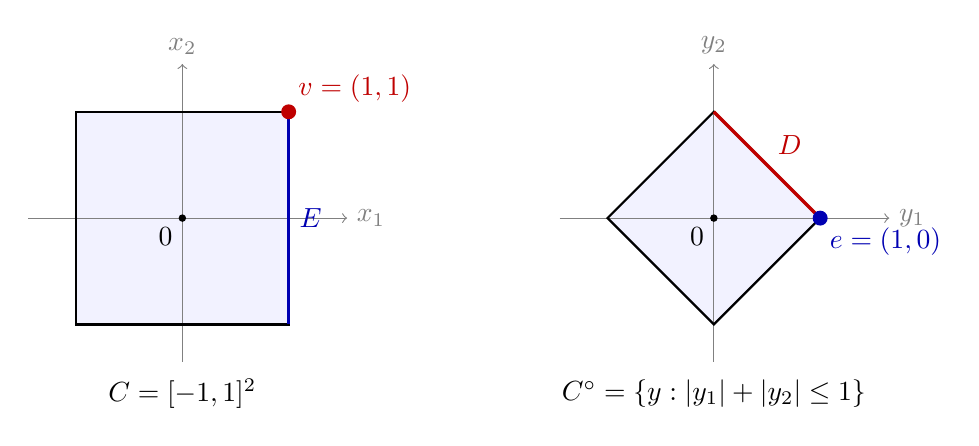
\begin{tikzpicture}[scale=1.35]
	\begin{scope}
		\fill[blue!5] (-1,-1) rectangle (1,1);
		\draw[->,gray] (-1.45,0)--(1.55,0) node[right] {\(x_1\)};
		\draw[->,gray] (0,-1.35)--(0,1.45) node[above] {\(x_2\)};
		\draw[thick] (-1,-1)--(1,-1)--(1,1)--(-1,1)--cycle;
		\draw[very thick,blue!70!black] (1,-1)--(1,1) node[midway,right] {\(E\)};
		\fill[red!75!black] (1,1) circle(2pt) node[above right] {\(v=(1,1)\)};
		\fill (0,0) circle(1pt) node[below left] {\(0\)};
		\node at (0,-1.65) {\(C=[-1,1]^2\)};
	\end{scope}
	\begin{scope}[xshift=5cm]
		\fill[blue!5] (1,0)--(0,1)--(-1,0)--(0,-1)--cycle;
		\draw[->,gray] (-1.45,0)--(1.65,0) node[right] {\(y_1\)};
		\draw[->,gray] (0,-1.35)--(0,1.45) node[above] {\(y_2\)};
		\draw[thick] (1,0)--(0,1)--(-1,0)--(0,-1)--cycle;
		\draw[very thick,red!75!black] (1,0)--(0,1) node[midway,above right] {\(D\)};
		\fill[blue!70!black] (1,0) circle(2pt) node[below right] {\(e=(1,0)\)};
		\fill (0,0) circle(1pt) node[below left] {\(0\)};
		\node at (0,-1.65) {\(C^\circ=\{y:|y_1|+|y_2|\le1\}\)};
	\end{scope}
\end{tikzpicture}

	\caption[正方形与极体的面对应]{正方形与极体的面对应。蓝边 \(E\) 对应蓝顶点 \(e\)；红顶点 \(v\) 对应红边 \(D\)。包含关系 \(v\in E\) 变为 \(e\in D\)。两幅图使用各自的坐标平面。}
	\label{g1:fig:square-polar}
\end{figure}

这种对应不仅存在于平面图形。原点位于内部时，每个支撑值都可以归一化成一，从而把一个面的外法向方向截成极体上的面。

\begin{proposition}[极体的面对应]
	\label{g1:prop:polar-face-duality}
	设 \(P\subseteq\mathbb R^d\) 为满维多胞形，且 \(0\in\operatorname{int}P\)。对非空真面 \(F\)，定义
	\[
		F^*=\{y\in P^\circ:\langle y,x\rangle=1\text{ 对所有 }x\in F\}.
	\]
	它是 \(P^\circ\) 的非空真面，且 \((F^*)^*=F\)。连同约定 \(P^*=\varnothing\)、\(\varnothing^*=P^\circ\)，这给出两个面格之间反转包含关系的双射。对非空真面还有
	\[
		\dim F+\dim F^*=d-1.
	\]
	特别地，顶点对应棱面，棱面对应顶点。
\end{proposition}

\begin{proof}
	选取线性函数 \(\langle u,-\rangle\) 暴露出 \(F\)，即 \(F=F_P(u)\)。因为 \(F\) 为真面，\(u\ne0\)；又因原点在内部，\(h_P(u)>0\)。于是 \(y_0=u/h_P(u)\) 属于 \(P^\circ\)，在 \(F\) 上配对为一，在其他顶点上配对严格小于一。这首先证明 \(F^*\ne\varnothing\)。取 \(F\) 全部顶点的平均点 \(x_0\)。对 \(y\in P^\circ\)，\(\langle y,x_0\rangle=1\) 当且仅当在 \(F\) 的每个顶点都配对为一，也就当且仅当在整个 \(F\) 上配对为一。因此
	\[
		F^*=\{y\in P^\circ:\langle y,x_0\rangle=1\}
	\]
	是一个暴露面。它不含 \(0\)，所以是一个真面。

	由双极公式，\((P^\circ)^\circ=P\)。按定义，\(F\subseteq(F^*)^*\)；若 \(x\in P\setminus F\)，刚才的 \(y_0\) 满足 \(\langle y_0,x\rangle<1\)，又有 \(y_0\in F^*\)，故 \(x\notin(F^*)^*\)。于是 \((F^*)^*=F\)。包含关系的反转直接来自条件“对所有 \(x\in F\)”；再对反向映射应用同一结论，得到反转包含的双射。空面与全体的约定也与包含关系相容。

	最后核对维数。设 \(k=\dim F\)，\(W\) 为 \(F\) 的仿射包络的方向空间，则 \(\dim W=k\)。因 \(F\) 位于支撑超平面 \(\langle y_0,x\rangle=1\) 中，\(x_0\notin W\)。所有对 \(F\) 配对为一的向量组成仿射空间
	\[
		Y=\{y:\langle y,x_0\rangle=1,\ \langle y,w\rangle=0\ (w\in W)\}.
	\]
	这些是 \(k+1\) 个独立线性条件，所以 \(\dim Y=d-k-1\)。在 \(y_0\) 附近、沿 \(Y\) 作足够小的扰动，对 \(F\) 的顶点仍配对为一；对有限个不在 \(F\) 中的顶点，由严格余量，配对仍小于一。因此 \(F^*\) 包含 \(y_0\) 在 \(Y\) 中的一个相对邻域，又完全位于 \(Y\) 内，故 \(\dim F^*=d-k-1\)。
\end{proof}

法锥与极体的面现在也可以直接比较：对非空真面 \(F\) 及 \(x_0\in F\)，有
\[
	F^*=N_P(F)\cap\{y:\langle y,x_0\rangle=1\},\qquad N_P(F)=\{ty:t\ge0,\ y\in F^*\}.
\]
第一个等式把最大值归一化；第二个等式使用了非零外法向量的支撑值严格为正。因而一个面先决定一整束外法向方向，再由极体从每条射线上选取一个代表。原点改变时，归一化的位置也会改变，极体不是单纯由图形的仿射外观决定的。

\subsection{单纯形、立方体和交叉多面体的对照}
\label{g1:subsec:0303:05}

取 \(d\ge2\)。记标准单纯形为 \(\Delta_d=\operatorname{conv}\{0,e_1,\ldots,e_d\}\)，将其重心移到原点后记为 \(S_d\)；另记
\[
	C_d=[-1,1]^d,\qquad O_d=\operatorname{conv}\{\pm e_1,\ldots,\pm e_d\}.
\]
其中 \(\Delta_d\) 是\secref{g1:sec:0101}已经定义的单纯形：它由 \(d+1\) 个仿射无关点生成，维数为 \(d\)。\(C_d\) 是 \(d\) 维立方体，\(O_d\) 称为\term[jiaochaduomianti]{交叉多面体}[cross-polytope]。平移单纯形只是为了满足取有界极体所需的原点条件，不改变其面及包含关系。

\begin{proposition}[三个模型的面数与对偶]
	\label{g1:prop:basic-polytope-counts}
	设 \(d\ge2\)，并以 \(f_k(P)\) 表示 \(P\) 的 \(k\) 维面的数目。则对 \(0\le k\le d-1\)，\cref{g1:tab:basic-polytopes}中的公式成立。其中 \(C_d^\circ=O_d\)、\(O_d^\circ=C_d\)，而 \(S_d^\circ\) 也是一个 \(d\) 维单纯形。
\end{proposition}

\begin{table}[htbp]
	\centering
	\caption[三个基本多胞形的计数与对偶]{三个基本多胞形的计数与对偶。\(0\le k\le d-1\)；每个多胞形另有一个空面和一个全体面。单纯形的极体记为 \(S'_d\)，不表示它与原单纯形逐点相同。}
	\label{g1:tab:basic-polytopes}
	\begin{tabular}{@{}lcccc@{}}
		\toprule
		对象 & 顶点数 & 棱面数 & \(f_k\) & 极体 \\
		\midrule
		单纯形 \(S_d\) & \(d+1\) & \(d+1\) & \(\binom{d+1}{k+1}\) & \(S'_d\) \\
		立方体 \(C_d\) & \(2^d\) & \(2d\) & \(2^{d-k}\binom dk\) & \(O_d\) \\
		交叉多面体 \(O_d\) & \(2d\) & \(2^d\) & \(2^{k+1}\binom d{k+1}\) & \(C_d\) \\
		\bottomrule
	\end{tabular}
\end{table}

\begin{proof}
	单纯形的每个非空面由一部分顶点生成；反过来，任意顶点子集都生成一个面。为说明后一点，使用单纯形上的重心坐标 \(\lambda_0,\ldots,\lambda_d\)：它们是仿射函数，非负且和为一。给定非空真子集 \(I\)，仿射函数 \(\sum_{i\in I}\lambda_i\) 的最大值为一，恰好在其余重心坐标全为零时取得，也就是选定顶点的凸包。仿射函数与其线性部分的最大值集相同，所以这确是一个暴露面。选出 \(k+1\) 个顶点便得到一个 \(k\) 维面，数目为 \(\binom{d+1}{k+1}\)。

	对于立方体，线性函数 \(\sum_i a_ix_i\) 取最大值时，\(a_i>0\) 迫使 \(x_i=1\)，\(a_i<0\) 迫使 \(x_i=-1\)，只有 \(a_i=0\) 的坐标可以自由变化。故 \(k\) 维面由 \(k\) 个自由坐标和其余坐标的 \(\pm1\) 选择确定，共有 \(\binom dk2^{d-k}\) 个。最大值本身是 \(\sum_i|a_i|\)，从而
	\[
		C_d^\circ=\{y:\textstyle\sum_i|y_i|\le1\}=O_d.
	\]
	最后一个等号可以直接核验：\(\sum_i|y_i|\le1\) 时，以 \(|y_i|\) 为系数使用相应符号的 \(e_i\)，剩余权重放在 \(0\)；而 \(0=(e_1+(-e_1))/2\) 本已在这些顶点的凸包中。双极公式给出 \(O_d^\circ=C_d\)。

	对于交叉多面体，非零线性函数 \(\langle a,-\rangle\) 的最大值为 \(M=\max_i|a_i|>0\)，达到最大值的顶点正是 \(\operatorname{sgn}(a_i)e_i\)、\(|a_i|=M\)。它们每个坐标方向至多选一个，且仿射无关。要得到 \(k\) 维面，应选 \(k+1\) 个坐标方向，每个方向任选正负号，共有 \(\binom d{k+1}2^{k+1}\) 种；每种确实能实现，只需让所选坐标的 \(a_i\) 等于相应的 \(\pm1\)，其余为零。

	还需确认平移单纯形的极体也是单纯形，而不只核对面数。置 \(b=(1/(d+1),\ldots,1/(d+1))\)，则 \(S_d=\Delta_d-b\)，故
	\[
		S_d=\{x:-(d+1)x_i\le1\ (1\le i\le d),\ (d+1)\textstyle\sum_i x_i\le1\}.
	\]
	记 \(q_i=-(d+1)e_i\) 和 \(q_0=(d+1)(1,\ldots,1)\)。这些 \(d+1\) 个点仿射无关，且平均为零：若 \(\sum_{i=1}^d c_i(q_i-q_0)=0\)，逐坐标得到 \(c_j=-\sum_i c_i\)，求和即迫使全部系数为零。因此 \(Q=\operatorname{conv}\{q_0,\ldots,q_d\}\) 是含原点的单纯形；上式恰好说明 \(Q^\circ=S_d\)。对闭凸含原点的 \(Q\) 应用双极公式，便有 \(S_d^\circ=Q\)。
\end{proof}

例如三维立方体有 \(8\) 个顶点、\(12\) 条棱和 \(6\) 个棱面，而三维交叉多面体即正八面体，分别有 \(6,12,8\) 个相应的面。两份数目倒序对应，反映的是 \(\dim F+\dim F^*=2\)，不是偶然的数字对称。在一维，单纯形、立方体和交叉多面体都只是线段；在零维，非空多胞形只有一个点，需要在零维环境中单独理解，不能把表中的棱面公式机械延伸过去。

有限表示、面格与极性还可以继续用于研究多胞形的组合结构。按这些主题延伸阅读，可查阅 \cite[Sections 1.1, 2.1--2.4]{Ziegler1995}。
